% Options for packages loaded elsewhere
\PassOptionsToPackage{unicode}{hyperref}
\PassOptionsToPackage{hyphens}{url}
%
\documentclass[
]{article}
\usepackage{amsmath,amssymb}
\usepackage{iftex}
\ifPDFTeX
  \usepackage[T1]{fontenc}
  \usepackage[utf8]{inputenc}
  \usepackage{textcomp} % provide euro and other symbols
\else % if luatex or xetex
  \usepackage{unicode-math} % this also loads fontspec
  \defaultfontfeatures{Scale=MatchLowercase}
  \defaultfontfeatures[\rmfamily]{Ligatures=TeX,Scale=1}
\fi
\usepackage{lmodern}
\ifPDFTeX\else
  % xetex/luatex font selection
\fi
% Use upquote if available, for straight quotes in verbatim environments
\IfFileExists{upquote.sty}{\usepackage{upquote}}{}
\IfFileExists{microtype.sty}{% use microtype if available
  \usepackage[]{microtype}
  \UseMicrotypeSet[protrusion]{basicmath} % disable protrusion for tt fonts
}{}
\makeatletter
\@ifundefined{KOMAClassName}{% if non-KOMA class
  \IfFileExists{parskip.sty}{%
    \usepackage{parskip}
  }{% else
    \setlength{\parindent}{0pt}
    \setlength{\parskip}{6pt plus 2pt minus 1pt}}
}{% if KOMA class
  \KOMAoptions{parskip=half}}
\makeatother
\usepackage{xcolor}
\usepackage[margin=1in]{geometry}
\usepackage{color}
\usepackage{fancyvrb}
\newcommand{\VerbBar}{|}
\newcommand{\VERB}{\Verb[commandchars=\\\{\}]}
\DefineVerbatimEnvironment{Highlighting}{Verbatim}{commandchars=\\\{\}}
% Add ',fontsize=\small' for more characters per line
\usepackage{framed}
\definecolor{shadecolor}{RGB}{248,248,248}
\newenvironment{Shaded}{\begin{snugshade}}{\end{snugshade}}
\newcommand{\AlertTok}[1]{\textcolor[rgb]{0.94,0.16,0.16}{#1}}
\newcommand{\AnnotationTok}[1]{\textcolor[rgb]{0.56,0.35,0.01}{\textbf{\textit{#1}}}}
\newcommand{\AttributeTok}[1]{\textcolor[rgb]{0.13,0.29,0.53}{#1}}
\newcommand{\BaseNTok}[1]{\textcolor[rgb]{0.00,0.00,0.81}{#1}}
\newcommand{\BuiltInTok}[1]{#1}
\newcommand{\CharTok}[1]{\textcolor[rgb]{0.31,0.60,0.02}{#1}}
\newcommand{\CommentTok}[1]{\textcolor[rgb]{0.56,0.35,0.01}{\textit{#1}}}
\newcommand{\CommentVarTok}[1]{\textcolor[rgb]{0.56,0.35,0.01}{\textbf{\textit{#1}}}}
\newcommand{\ConstantTok}[1]{\textcolor[rgb]{0.56,0.35,0.01}{#1}}
\newcommand{\ControlFlowTok}[1]{\textcolor[rgb]{0.13,0.29,0.53}{\textbf{#1}}}
\newcommand{\DataTypeTok}[1]{\textcolor[rgb]{0.13,0.29,0.53}{#1}}
\newcommand{\DecValTok}[1]{\textcolor[rgb]{0.00,0.00,0.81}{#1}}
\newcommand{\DocumentationTok}[1]{\textcolor[rgb]{0.56,0.35,0.01}{\textbf{\textit{#1}}}}
\newcommand{\ErrorTok}[1]{\textcolor[rgb]{0.64,0.00,0.00}{\textbf{#1}}}
\newcommand{\ExtensionTok}[1]{#1}
\newcommand{\FloatTok}[1]{\textcolor[rgb]{0.00,0.00,0.81}{#1}}
\newcommand{\FunctionTok}[1]{\textcolor[rgb]{0.13,0.29,0.53}{\textbf{#1}}}
\newcommand{\ImportTok}[1]{#1}
\newcommand{\InformationTok}[1]{\textcolor[rgb]{0.56,0.35,0.01}{\textbf{\textit{#1}}}}
\newcommand{\KeywordTok}[1]{\textcolor[rgb]{0.13,0.29,0.53}{\textbf{#1}}}
\newcommand{\NormalTok}[1]{#1}
\newcommand{\OperatorTok}[1]{\textcolor[rgb]{0.81,0.36,0.00}{\textbf{#1}}}
\newcommand{\OtherTok}[1]{\textcolor[rgb]{0.56,0.35,0.01}{#1}}
\newcommand{\PreprocessorTok}[1]{\textcolor[rgb]{0.56,0.35,0.01}{\textit{#1}}}
\newcommand{\RegionMarkerTok}[1]{#1}
\newcommand{\SpecialCharTok}[1]{\textcolor[rgb]{0.81,0.36,0.00}{\textbf{#1}}}
\newcommand{\SpecialStringTok}[1]{\textcolor[rgb]{0.31,0.60,0.02}{#1}}
\newcommand{\StringTok}[1]{\textcolor[rgb]{0.31,0.60,0.02}{#1}}
\newcommand{\VariableTok}[1]{\textcolor[rgb]{0.00,0.00,0.00}{#1}}
\newcommand{\VerbatimStringTok}[1]{\textcolor[rgb]{0.31,0.60,0.02}{#1}}
\newcommand{\WarningTok}[1]{\textcolor[rgb]{0.56,0.35,0.01}{\textbf{\textit{#1}}}}
\usepackage{graphicx}
\makeatletter
\def\maxwidth{\ifdim\Gin@nat@width>\linewidth\linewidth\else\Gin@nat@width\fi}
\def\maxheight{\ifdim\Gin@nat@height>\textheight\textheight\else\Gin@nat@height\fi}
\makeatother
% Scale images if necessary, so that they will not overflow the page
% margins by default, and it is still possible to overwrite the defaults
% using explicit options in \includegraphics[width, height, ...]{}
\setkeys{Gin}{width=\maxwidth,height=\maxheight,keepaspectratio}
% Set default figure placement to htbp
\makeatletter
\def\fps@figure{htbp}
\makeatother
\setlength{\emergencystretch}{3em} % prevent overfull lines
\providecommand{\tightlist}{%
  \setlength{\itemsep}{0pt}\setlength{\parskip}{0pt}}
\setcounter{secnumdepth}{-\maxdimen} % remove section numbering
\ifLuaTeX
  \usepackage{selnolig}  % disable illegal ligatures
\fi
\usepackage{bookmark}
\IfFileExists{xurl.sty}{\usepackage{xurl}}{} % add URL line breaks if available
\urlstyle{same}
\hypersetup{
  pdftitle={BIOS 731 Homework 4},
  pdfauthor={Linlin Wu},
  hidelinks,
  pdfcreator={LaTeX via pandoc}}

\title{BIOS 731 Homework 4}
\author{Linlin Wu}
\date{2026-03-27}

\begin{document}
\maketitle

\section{Problem 1: Gibbs sampler derivations and
implementation}\label{problem-1-gibbs-sampler-derivations-and-implementation}

We consider the Bayesian mixture model \[
\mu_k \sim N(0,\sigma^2), \quad k = 1,\dots,K,
\] \[
c_i \sim \text{Categorical}(1/K,\dots,1/K), \quad i = 1,\dots,n,
\] \[
y_i \mid c_i,\mu \sim N(\mu_{c_i}, 1).
\]

The goal is to derive a Gibbs sampler for the posterior distribution
\(p(\mu, c \mid y)\), and then implement it in R.

\subsection{\texorpdfstring{Derivation of
\(p(c_i \mid y_i, \mu)\)}{Derivation of p(c\_i \textbackslash mid y\_i, \textbackslash mu)}}\label{derivation-of-pc_i-mid-y_i-mu}

Conditioning on \(\mu\), the full conditional distribution of \(c_i\) is
\[
p(c_i = k \mid y_i, \mu)
\propto p(y_i \mid c_i = k, \mu)\, p(c_i = k).
\]

Since the prior on \(c_i\) is uniform over \(1,\dots,K\), \[
p(c_i = k) = \frac{1}{K},
\] which is constant in \(k\). Therefore, \[
p(c_i = k \mid y_i, \mu)
\propto \exp\left\{-\frac12 (y_i - \mu_k)^2\right\}.
\]

After normalization, \[
p(c_i = k \mid y_i, \mu)
=
\frac{\exp\left\{-\frac12 (y_i - \mu_k)^2\right\}}
{\sum_{\ell=1}^K \exp\left\{-\frac12 (y_i - \mu_\ell)^2\right\}}.
\]

Thus, \[
c_i \mid y_i, \mu \sim \text{Categorical}(\pi_{i1},\dots,\pi_{iK}),
\] where \[
\pi_{ik}
=
\frac{\exp\left\{-\frac12 (y_i - \mu_k)^2\right\}}
{\sum_{\ell=1}^K \exp\left\{-\frac12 (y_i - \mu_\ell)^2\right\}}.
\]

\subsection{\texorpdfstring{Derivation of
\(p(\mu_k \mid y, c)\)}{Derivation of p(\textbackslash mu\_k \textbackslash mid y, c)}}\label{derivation-of-pmu_k-mid-y-c}

Let \[
n_k = \sum_{i=1}^n I(c_i = k)
\] and \[
S_k = \sum_{i:c_i=k} y_i.
\]

The full conditional of \(\mu_k\) is proportional to the prior times the
likelihood contributions from observations assigned to cluster \(k\): \[
p(\mu_k \mid y, c)
\propto
\exp\left(-\frac{\mu_k^2}{2\sigma^2}\right)
\prod_{i:c_i=k}\exp\left\{-\frac12 (y_i-\mu_k)^2\right\}.
\]

Taking logs and collecting terms in \(\mu_k\), \[
\log p(\mu_k \mid y, c)
=
-\frac12
\left[
\left(n_k + \frac{1}{\sigma^2}\right)\mu_k^2
- 2S_k\mu_k
\right]
+ \text{const}.
\]

This is the kernel of a normal density. Therefore, \[
\mu_k \mid y,c \sim N(m_k, v_k),
\] where \[
v_k = \left(n_k + \frac{1}{\sigma^2}\right)^{-1},
\qquad
m_k = v_k S_k.
\]

Equivalently, \[
m_k
=
\frac{\sum_{i:c_i=k} y_i}{n_k + 1/\sigma^2}.
\]

If \(n_k = 0\), then \(S_k = 0\) and the update reduces to the prior \[
\mu_k \mid y,c \sim N(0,\sigma^2).
\]

\subsubsection{Gibbs sampler updates}\label{gibbs-sampler-updates}

The Gibbs sampler alternates between the following two steps:

\begin{enumerate}
\def\labelenumi{\arabic{enumi}.}
\item
  For each \(i=1,\dots,n\), sample \[
  c_i \mid y_i,\mu \sim \text{Categorical}(\pi_{i1},\dots,\pi_{iK}).
  \]
\item
  For each \(k=1,\dots,K\), sample \[
  \mu_k \mid y,c \sim N(m_k,v_k).
  \]
\end{enumerate}

I implemented these updates in \texttt{source/p1\_gibbs\_functions.R},
and then ran the sampler using \texttt{source/p1\_gibbs\_run.R}. The
script stores posterior draws and saves summary results and figures to
the \texttt{results/} folder.

\subsubsection{Implementation check on simulated
data}\label{implementation-check-on-simulated-data}

As a quick implementation check, I simulated data from a 3-component
Gaussian mixture with true means \((-3, 0, 4)\), and then ran the Gibbs
sampler with \(4000\) iterations and burn-in \(1000\).

\begin{Shaded}
\begin{Highlighting}[]
\NormalTok{fit\_gibbs }\OtherTok{\textless{}{-}} \FunctionTok{readRDS}\NormalTok{(}\StringTok{"../results/p1\_fit\_gibbs.rds"}\NormalTok{)}
\NormalTok{mu\_summary }\OtherTok{\textless{}{-}} \FunctionTok{read.csv}\NormalTok{(}\StringTok{"../results/p1\_mu\_post\_mean.csv"}\NormalTok{)}
\NormalTok{cluster\_summary }\OtherTok{\textless{}{-}} \FunctionTok{read.csv}\NormalTok{(}\StringTok{"../results/p1\_cluster\_summary.csv"}\NormalTok{)}
\NormalTok{mu\_summary}
\end{Highlighting}
\end{Shaded}

\begin{verbatim}
##   component posterior_mean
## 1       mu1    -3.29088597
## 2       mu2    -0.06404715
## 3       mu3     3.96163103
\end{verbatim}

The posterior mean estimates of the component means are:

\begin{Shaded}
\begin{Highlighting}[]
\FunctionTok{round}\NormalTok{(fit\_gibbs}\SpecialCharTok{$}\NormalTok{mu\_post\_mean, }\DecValTok{3}\NormalTok{)}
\end{Highlighting}
\end{Shaded}

\begin{verbatim}
## [1] -3.291 -0.064  3.962
\end{verbatim}

The trace plots for the component means are shown below.

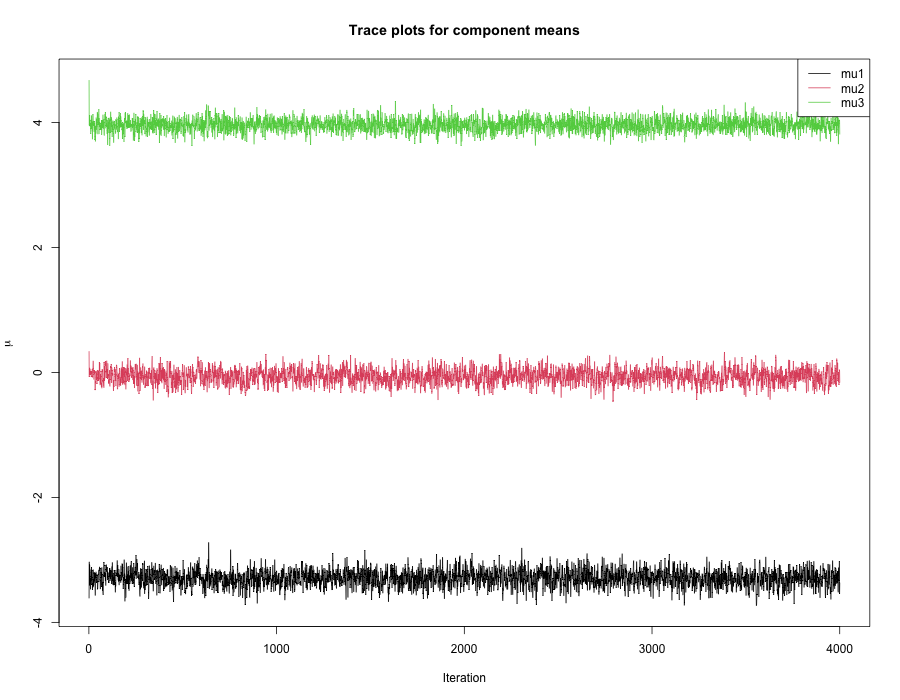
\includegraphics[width=0.8\linewidth]{../results/p1_traceplot}

A posterior summary for the estimated cluster assignments is given by
the posterior mode of each \(c_i\).

\begin{Shaded}
\begin{Highlighting}[]
\NormalTok{cluster\_summary}
\end{Highlighting}
\end{Shaded}

\begin{verbatim}
##   cluster count
## 1       1    82
## 2       2   108
## 3       3   110
\end{verbatim}

The posterior mean estimates are close to the true values used in
simulation, and the trace plots appear stable over iterations. This
suggests that the Gibbs sampler was implemented correctly for this
problem.

\section{Problem 2: Variational inference
derivations}\label{problem-2-variational-inference-derivations}

For Problem 2, I use a mean-field variational approximation to the
posterior distribution \[
p(\mu, c \mid y),
\] where the variational family is \[
q(\mu, c)
=
\prod_{k=1}^K q(\mu_k)\prod_{i=1}^n q(c_i).
\]

I assume \[
q(\mu_k) = N(m_k, s_k^2),
\qquad
q(c_i) = \text{Categorical}(\phi_{i1}, \dots, \phi_{iK}),
\] where \(\sum_{k=1}^K \phi_{ik} = 1\) for each \(i\).

\subsection{Joint log-density}\label{joint-log-density}

Ignoring constants that do not depend on \(\mu\) or \(c\), the
complete-data log-density is \[
\log p(y, c, \mu)
=
\sum_{k=1}^K \log p(\mu_k)
+
\sum_{i=1}^n \log p(c_i)
+
\sum_{i=1}^n \log p(y_i \mid c_i, \mu).
\]

Under the model, \[
\log p(\mu_k)
=
-\frac12 \log(2\pi \sigma^2) - \frac{\mu_k^2}{2\sigma^2},
\] \[
\log p(c_i = k) = \log(1/K),
\] and \[
\log p(y_i \mid c_i = k, \mu)
=
-\frac12 \log(2\pi) - \frac12 (y_i - \mu_k)^2.
\]

\subsection{\texorpdfstring{Update for
\(q(c_i)\)}{Update for q(c\_i)}}\label{update-for-qc_i}

Using the standard CAVI formula, \[
\log q^*(c_i)
=
\mathbb{E}_{q(\mu)}[\log p(y, c, \mu)] + \text{const},
\] where only the terms involving \(c_i\) are needed. For
\(k = 1,\dots,K\), \[
\log q^*(c_i = k)
=
\mathbb{E}_{q(\mu_k)}[\log p(y_i \mid c_i = k, \mu_k)]
+ \log p(c_i = k)
+ \text{const}.
\]

Because \[
\mathbb{E}_{q(\mu_k)}[(y_i - \mu_k)^2]
=
y_i^2 - 2 y_i m_k + (m_k^2 + s_k^2),
\] we obtain \[
\log q^*(c_i = k)
=
-\frac12\left[y_i^2 - 2y_i m_k + (m_k^2 + s_k^2)\right]
+ \log(1/K)
+ \text{const}.
\]

Dropping terms that do not depend on \(k\), \[
\log q^*(c_i = k)
=
y_i m_k - \frac12(m_k^2 + s_k^2) + \text{const}.
\]

Therefore, \[
\phi_{ik}
\propto
\exp\left\{
y_i m_k - \frac12(m_k^2 + s_k^2)
\right\},
\] and after normalization, \[
\phi_{ik}
=
\frac{
\exp\left\{
y_i m_k - \frac12(m_k^2 + s_k^2)
\right\}
}{
\sum_{\ell=1}^K
\exp\left\{
y_i m_\ell - \frac12(m_\ell^2 + s_\ell^2)
\right\}
}.
\]

\subsection{\texorpdfstring{Update for
\(q(\mu_k)\)}{Update for q(\textbackslash mu\_k)}}\label{update-for-qmu_k}

Again using the CAVI formula, \[
\log q^*(\mu_k)
=
\mathbb{E}_{q(c), q(\mu_{-k})}[\log p(y, c, \mu)] + \text{const}.
\]

Keeping only terms involving \(\mu_k\), \[
\log q^*(\mu_k)
=
-\frac{\mu_k^2}{2\sigma^2}
-\frac12 \sum_{i=1}^n \phi_{ik}(y_i - \mu_k)^2
+ \text{const}.
\]

Expand the quadratic term: \[
\log q^*(\mu_k)
=
-\frac12
\left[
\left(\frac{1}{\sigma^2} + \sum_{i=1}^n \phi_{ik}\right)\mu_k^2
- 2\left(\sum_{i=1}^n \phi_{ik} y_i\right)\mu_k
\right]
+ \text{const}.
\]

So \(q(\mu_k)\) is Gaussian: \[
q(\mu_k) = N(m_k, s_k^2),
\] with \[
s_k^2
=
\left(\frac{1}{\sigma^2} + \sum_{i=1}^n \phi_{ik}\right)^{-1},
\qquad
m_k
=
s_k^2 \sum_{i=1}^n \phi_{ik} y_i.
\]

\subsection{ELBO}\label{elbo}

To monitor convergence, I evaluate the evidence lower bound \[
\text{ELBO}(q)
=
\mathbb{E}_q[\log p(y, c, \mu)]
-
\mathbb{E}_q[\log q(c, \mu)].
\]

In the implementation, this is computed as the sum of five parts:

\begin{enumerate}
\def\labelenumi{\arabic{enumi}.}
\tightlist
\item
  \(\mathbb{E}_q[\log p(\mu)]\)
\item
  \(\mathbb{E}_q[\log p(c)]\)
\item
  \(\mathbb{E}_q[\log p(y \mid c,\mu)]\)
\item
  entropy of \(q(c)\)
\item
  entropy of \(q(\mu)\)
\end{enumerate}

The CAVI algorithm iterates between updating \(\phi\), \(m\), and
\(s^2\) until the ELBO stabilizes.

\subsection{R implementation}\label{r-implementation}

I implemented the variational updates in
\texttt{source/p2\_vi\_functions.R} and ran them in
\texttt{source/p2\_vi\_run.R}. The algorithm stores the ELBO path,
returns final estimates of the cluster assignments and means, and saves
the numerical summaries and plots to the \texttt{results/} folder, as
required. :contentReference{oaicite:1}

\subsection{Implementation check on simulated
data}\label{implementation-check-on-simulated-data-1}

As a quick implementation check, I again simulated data from a
3-component Gaussian mixture with true means \((-3, 0, 4)\), and then
ran the CAVI algorithm.

\begin{Shaded}
\begin{Highlighting}[]
\NormalTok{fit\_vi }\OtherTok{\textless{}{-}} \FunctionTok{readRDS}\NormalTok{(}\StringTok{"../results/p2\_fit\_vi.rds"}\NormalTok{)}
\NormalTok{mu\_summary\_vi }\OtherTok{\textless{}{-}} \FunctionTok{read.csv}\NormalTok{(}\StringTok{"../results/p2\_mu\_summary.csv"}\NormalTok{)}
\NormalTok{cluster\_summary\_vi }\OtherTok{\textless{}{-}} \FunctionTok{read.csv}\NormalTok{(}\StringTok{"../results/p2\_cluster\_summary.csv"}\NormalTok{)}
\FunctionTok{head}\NormalTok{(}\FunctionTok{read.csv}\NormalTok{(}\StringTok{"../results/p2\_elbo.csv"}\NormalTok{))}
\end{Highlighting}
\end{Shaded}

\begin{verbatim}
##   iteration      elbo
## 1         1 -755.3068
## 2         2 -725.4166
## 3         3 -722.7223
## 4         4 -722.3078
## 5         5 -722.2210
## 6         6 -722.2018
\end{verbatim}

The final variational estimates of the component means are:

\begin{Shaded}
\begin{Highlighting}[]
\FunctionTok{round}\NormalTok{(fit\_vi}\SpecialCharTok{$}\NormalTok{m, }\DecValTok{3}\NormalTok{)}
\end{Highlighting}
\end{Shaded}

\begin{verbatim}
## [1] -3.294 -0.064  3.958
\end{verbatim}

The ELBO path is shown below.

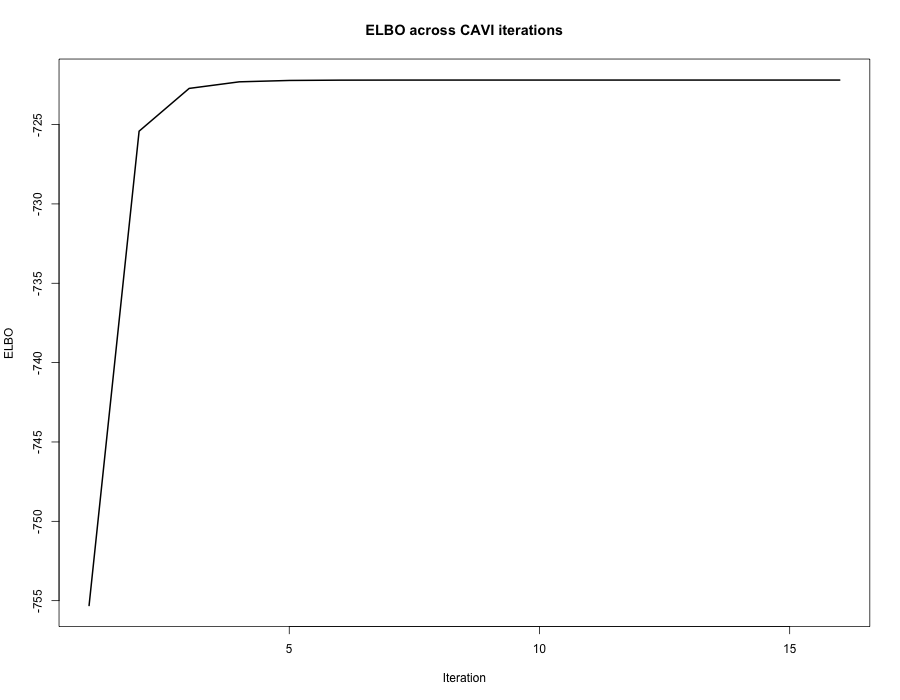
\includegraphics[width=0.8\linewidth]{../results/p2_elbo_plot}

A posterior summary for the estimated cluster assignments is given by
assigning each observation to the component with the largest variational
probability \(\phi_{ik}\).

\begin{Shaded}
\begin{Highlighting}[]
\NormalTok{cluster\_summary\_vi}
\end{Highlighting}
\end{Shaded}

\begin{verbatim}
##   cluster count
## 1       1    82
## 2       2   108
## 3       3   110
\end{verbatim}

The ELBO increases monotonically and then stabilizes after a small
number of iterations, which is consistent with convergence of the CAVI
algorithm. The final variational mean estimates, (−3.294,−0.064,3.958),
are also close to the true component means used in the simulated
example, suggesting that the implementation is correct.

\section{Problem 3: Fit to data}\label{problem-3-fit-to-data}

In this problem, I fit both the Gibbs sampler and the variational
inference algorithm to the Old Faithful waiting times data, and then
compare their computation times and parameter estimates. For the Gibbs
sampler, I also run multiple chains and examine diagnostic plots,
convergence, and effective sample size, as required.
:contentReference{oaicite:1}

I use the waiting-time variable from the built-in \texttt{faithful}
dataset and fit a 2-component Gaussian mixture model, which is
appropriate for the clearly bimodal structure of these waiting times.

\subsection{Data}\label{data}

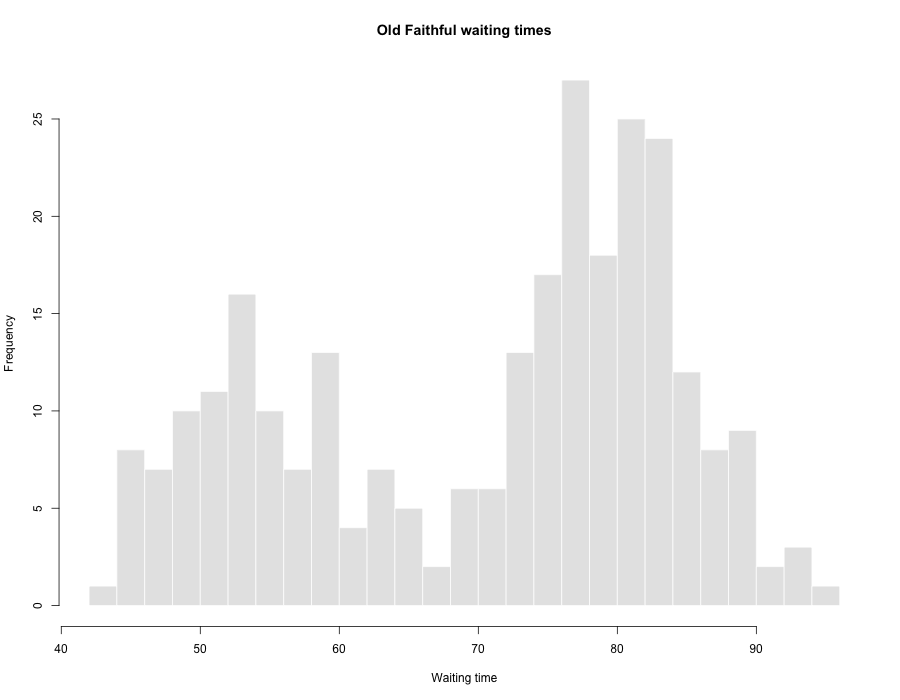
\includegraphics[width=0.75\linewidth]{../results/p3_oldfaithful_hist}

\subsection{Model fitting}\label{model-fitting}

For Gibbs sampling, I ran 4 chains, each with 10,000 iterations and a
burn-in of 2,000. For variational Bayes, I ran the CAVI algorithm until
the ELBO converged. The required comparison focuses on computation time
and mean estimates from the two methods. :contentReference{oaicite:2}

\begin{Shaded}
\begin{Highlighting}[]
\NormalTok{timing\_summary\_p3 }\OtherTok{\textless{}{-}} \FunctionTok{read.csv}\NormalTok{(}\StringTok{"../results/p3\_timing\_summary.csv"}\NormalTok{)}
\NormalTok{estimate\_summary\_p3 }\OtherTok{\textless{}{-}} \FunctionTok{read.csv}\NormalTok{(}\StringTok{"../results/p3\_estimate\_summary.csv"}\NormalTok{)}
\NormalTok{diag\_summary\_p3 }\OtherTok{\textless{}{-}} \FunctionTok{read.csv}\NormalTok{(}\StringTok{"../results/p3\_gibbs\_diagnostics.csv"}\NormalTok{)}
\NormalTok{gibbs\_cluster\_summary\_p3 }\OtherTok{\textless{}{-}} \FunctionTok{read.csv}\NormalTok{(}\StringTok{"../results/p3\_gibbs\_cluster\_summary.csv"}\NormalTok{)}
\NormalTok{vi\_cluster\_summary\_p3 }\OtherTok{\textless{}{-}} \FunctionTok{read.csv}\NormalTok{(}\StringTok{"../results/p3\_vi\_cluster\_summary.csv"}\NormalTok{)}

\NormalTok{timing\_summary\_p3}
\end{Highlighting}
\end{Shaded}

\begin{verbatim}
##                method elapsed_seconds
## 1 Gibbs_total_4chains          29.928
## 2 Gibbs_avg_per_chain           7.482
## 3                  VI           0.001
\end{verbatim}

\subsection{Comparison of estimates and computation
times}\label{comparison-of-estimates-and-computation-times}

The estimated component means from Gibbs sampling and variational Bayes
are:

\begin{Shaded}
\begin{Highlighting}[]
\NormalTok{estimate\_summary\_p3}
\end{Highlighting}
\end{Shaded}

\begin{verbatim}
##   parameter gibbs_posterior_mean  vi_mean
## 1       mu1             54.74436 54.74453
## 2       mu2             80.28038 80.28022
\end{verbatim}

The cluster-size summaries based on the final posterior summaries are:

\begin{Shaded}
\begin{Highlighting}[]
\NormalTok{gibbs\_cluster\_summary\_p3}
\end{Highlighting}
\end{Shaded}

\begin{verbatim}
##   cluster count
## 1       1   100
## 2       2   172
\end{verbatim}

\begin{Shaded}
\begin{Highlighting}[]
\NormalTok{vi\_cluster\_summary\_p3}
\end{Highlighting}
\end{Shaded}

\begin{verbatim}
##   cluster count
## 1       1   100
## 2       2   172
\end{verbatim}

The timing comparison is:

\begin{Shaded}
\begin{Highlighting}[]
\NormalTok{timing\_summary\_p3}
\end{Highlighting}
\end{Shaded}

\begin{verbatim}
##                method elapsed_seconds
## 1 Gibbs_total_4chains          29.928
## 2 Gibbs_avg_per_chain           7.482
## 3                  VI           0.001
\end{verbatim}

\subsection{Gibbs sampler diagnostics}\label{gibbs-sampler-diagnostics}

The following trace plots show the Gibbs sampler output across the 4
chains for each component mean.

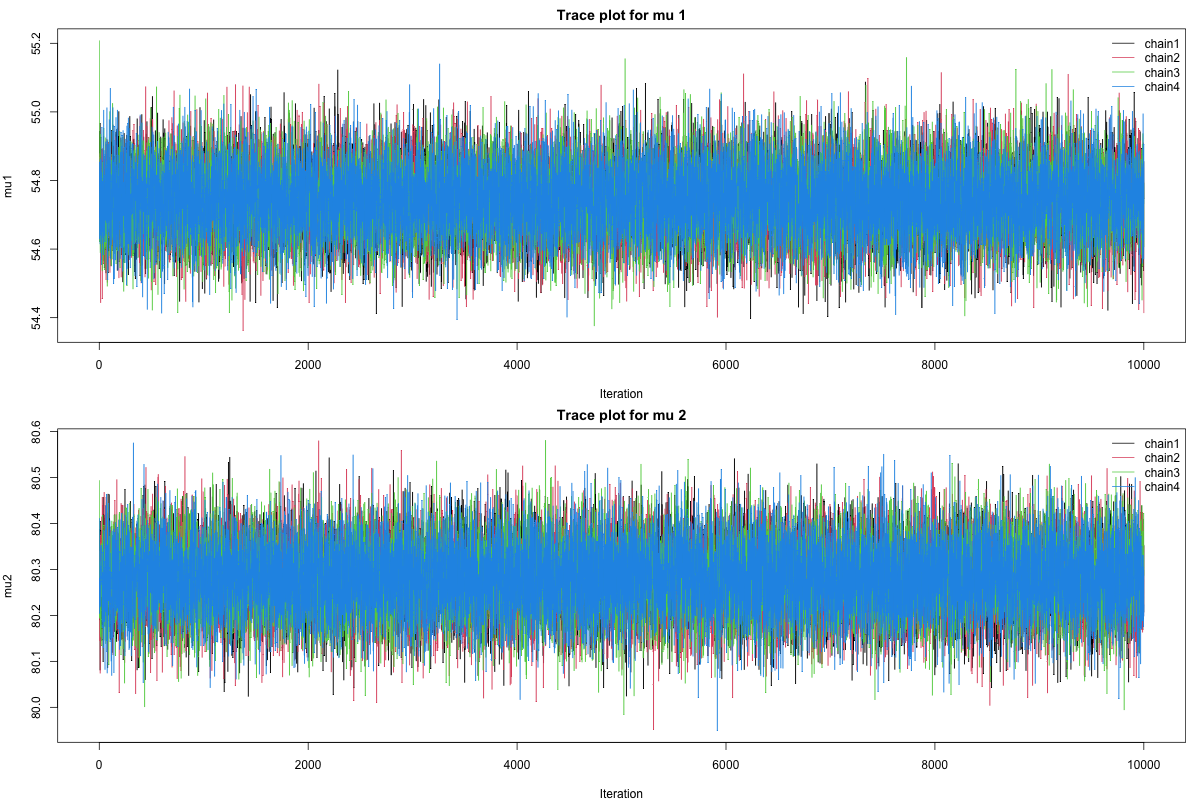
\includegraphics[width=0.85\linewidth]{../results/p3_gibbs_traceplot}

The following ACF plots are based on the post-burn-in samples from chain
1.

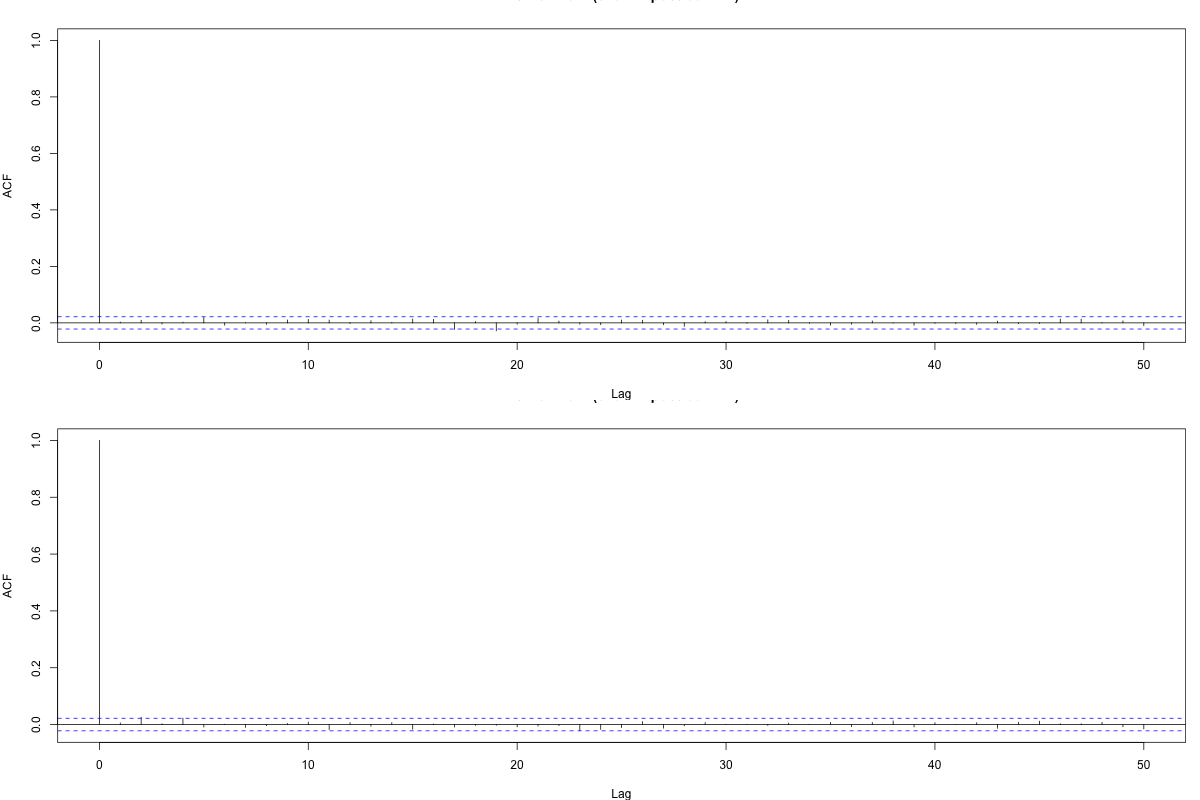
\includegraphics[width=0.85\linewidth]{../results/p3_gibbs_acf}

To assess convergence more formally, I compute \(\hat{R}\) and effective
sample size for each component mean.

\begin{Shaded}
\begin{Highlighting}[]
\NormalTok{diag\_summary\_p3}
\end{Highlighting}
\end{Shaded}

\begin{verbatim}
##   parameter      ess      rhat
## 1       mu1 32539.99 0.9999886
## 2       mu2 30665.90 1.0001718
\end{verbatim}

The \(\hat{R}\) values close to 1 indicate that the multiple Gibbs
chains mixed well and converged to a common posterior distribution. The
effective sample sizes summarize the amount of usable posterior
information after accounting for autocorrelation.

\subsection{Variational inference
convergence}\label{variational-inference-convergence}

The ELBO path for the variational fit is shown below.

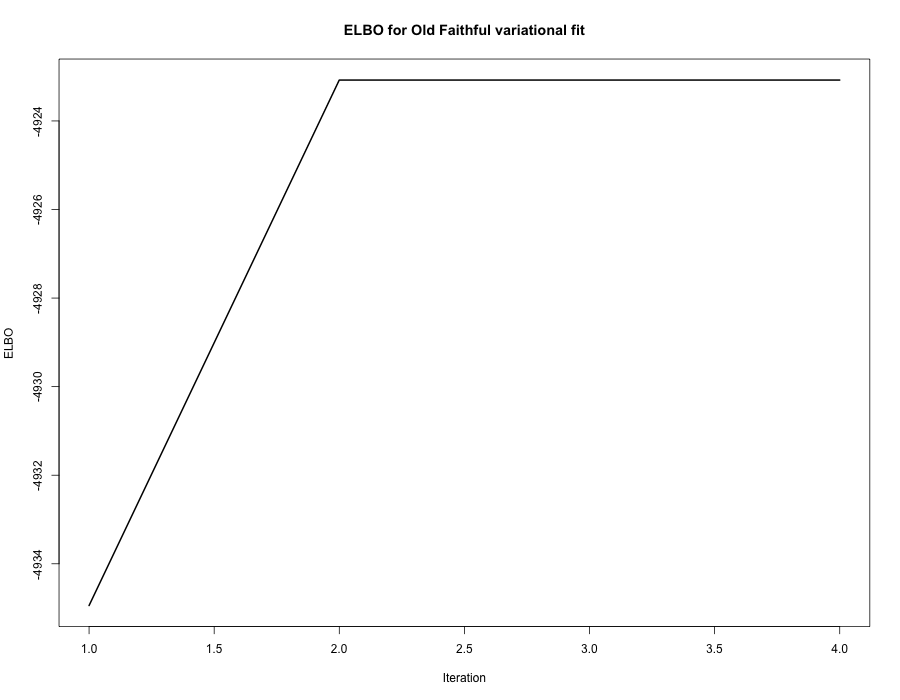
\includegraphics[width=0.75\linewidth]{../results/p3_vi_elbo}

\subsection{Comments}\label{comments}

Overall, both methods produced very similar estimates for the two
component means. The Gibbs posterior means were 54.74 and 80.28, while
the corresponding variational Bayes estimates were 54.75 and 80.28.
Thus, for this dataset, variational Bayes provided an excellent
approximation to the posterior mean estimates from Gibbs sampling. In
terms of computation, variational Bayes was much faster than Gibbs
sampling. For the Gibbs sampler, the trace plots showed stable mixing
across chains, the \hat{R} values were essentially 1, and the effective
sample sizes were large, all of which support good convergence.

\end{document}
